%!TEX root = ../scivis_lbaakman_bvanloon.tex
This section discusses the colormaps provided in the application. Each colormap is accompanied with a short discussion giving the main goal of the colormap and its pros and cons.

As discussed in the previous section, colormaps provide a way to map scalar values to colors in order for the user to extract information. The quality of a colormap can be judged by how well and intuitive the colormap allows inverse mapping. Which colormap is best used depends on the context and goal of the visualization. The zebra-colormap is for example well suited to visualize value variations (i.e. the first derivative of a scalar value), but would be less useful would the aim be to highlight maxima. Historical reasons can also influence the choice of colormaps. X-rays are for example standard displayed using a gray-scale colormap. Better alternatives might exist, but are not used due to status quo in the medical field.

In our application we have chosen to implement a variety of colormaps, this way the application offers a suitable colormap for almost any form of visualization, ranging from the (in)famous rainbow colormap to luminance based, two-hue and diverging colormaps.

\begin{figure}[b]
	\begin{subfigure}{1\textwidth}
		\begin{minipage}[l]{0.05\textwidth}
	    	\caption{} \label{fig:colormaps:legends:rainbow}
	  	\end{minipage}
	  \hfill
	  	\begin{minipage}[l]{0.95\textwidth}
	    	
\includegraphics[width=\textwidth,height=15px,keepaspectratio=false,frame]{colormapping/img/colormap_legends/rainbowcolormap.png}
	  	\end{minipage}
	\end{subfigure}

  	\begin{subfigure}{1\textwidth}
  		\begin{minipage}[l]{0.05\textwidth}
    		\caption{} \label{fig:colormaps:legends::zebra}
  		\end{minipage}
  	\hfill
  		\begin{minipage}[l]{0.95\textwidth}
    		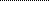
\includegraphics[width=\textwidth,height=15px,keepaspectratio=false,frame]{colormapping/img/colormap_legends/zebracolormap.png}
  		\end{minipage}
  	\end{subfigure}

  	\begin{subfigure}{1\textwidth}
  		\begin{minipage}[l]{0.05\textwidth}
    		\caption{} \label{fig:colormaps:legends::grayscale}
  		\end{minipage}
  	\hfill
  		\begin{minipage}[l]{0.95\textwidth}
    		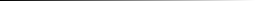
\includegraphics[width=\textwidth,height=15px,keepaspectratio=false,frame]{colormapping/img/colormap_legends/grayscalecolormap.png}
  		\end{minipage}
  	\end{subfigure}
  	\begin{subfigure}{1\textwidth}
  		\begin{minipage}[l]{0.05\textwidth}
    		\caption{} \label{fig:colormaps:legends::heat}
  		\end{minipage}
  	\hfill
  		\begin{minipage}[l]{0.95\textwidth}
    		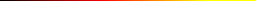
\includegraphics[width=\textwidth,height=15px,keepaspectratio=false,frame]{colormapping/img/colormap_legends/heatcolormap.png}
  		\end{minipage}
  	\end{subfigure}
  	\begin{subfigure}{1\textwidth}
  		\begin{minipage}[l]{0.05\textwidth}
    		\caption{} \label{fig:colormaps:legends::cold}
  		\end{minipage}
  	\hfill
  		\begin{minipage}[l]{0.95\textwidth}
    		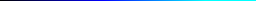
\includegraphics[width=\textwidth,height=15px,keepaspectratio=false,frame]{colormapping/img/colormap_legends/coldcolormap.png}
  		\end{minipage}
  	\end{subfigure}
  	\begin{subfigure}{1\textwidth}
  		\begin{minipage}[l]{0.05\textwidth}
    		\caption{} \label{fig:colormaps:legends::hue}
  		\end{minipage}
  	\hfill
  		\begin{minipage}[l]{0.95\textwidth}
    		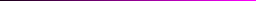
\includegraphics[width=\textwidth,height=15px,keepaspectratio=false,frame]{colormapping/img/colormap_legends/huecolormap.png}
  		\end{minipage}
  	\end{subfigure}
  	\begin{subfigure}{1\textwidth}
  		\begin{minipage}[l]{0.05\textwidth}
    		\caption{} \label{fig:colormaps:legends::twocolors}
  		\end{minipage}
  	\hfill
  		\begin{minipage}[l]{0.95\textwidth}
    		
\includegraphics[width=\textwidth,height=15px,keepaspectratio=false,frame]{colormapping/img/colormap_legends/twocolorscolormap.png}
  		\end{minipage}
  	\end{subfigure}
  	\begin{subfigure}{1\textwidth}
  		\begin{minipage}[l]{0.05\textwidth}
    		\caption{} \label{fig:colormaps:legends::diverging}
  		\end{minipage}
  	\hfill
  		\begin{minipage}[l]{0.95\textwidth}
    		
\includegraphics[width=\textwidth,height=15px,keepaspectratio=false,frame]{colormapping/img/colormap_legends/divergingcolormap.png}
  		\end{minipage}
  	\end{subfigure}
\caption{Colormap legends provided in the application: 
(\subref{fig:colormaps:legends:rainbow}) rainbow, 
\subref{fig:colormaps:legends::zebra} zebra,
\subref{fig:colormaps:legends::grayscale} gray-scale,
\subref{fig:colormaps:legends::heat} heat,
\subref{fig:colormaps:legends::cold} cold,
\subref{fig:colormaps:legends::hue} user picked hue,
\subref{fig:colormaps:legends::twocolors} linear two-color, and
\subref{fig:colormaps:legends::diverging} blue-red diverging. Each colormap is shown using full saturation and 256 colors (except for the zebra map which has 50 color regions). 
 }\label{fig:colormaps:legends}
\end{figure}


\subsection{Rainbow Colormap} % (fold)
\label{ssub:rainbow_colormap}
The rainbow colormap (given in \cref{fig:colormaps:legends:rainbow}) is one of the most used colormaps in the scientific community and is therefore included in our application. The colormap is constructed by first doing a piecewise interpolation of blue to green and next from green to red. The resulting colors in the colormaps are a mix of blue and green or a mix of green and red, except for the tails of the colormap which contain only blue or red.

The colormap is often seen as visual appealing due to the varying colors and can give an intuitively mapping of high and low values to warm (red) and cold (blue) colors. However, although often used, the rainbow colormap has many flaws and is heavily critiqued\cite{borland2007rainbow}\cite{divergingMoreland2009}. A few of the most serious flaws are discussed below.
\begin{itemize}
  \item The rainbow colormap pulls the focus of users towards areas with high values (and thus warm, red colors). This can be an advantage when the area of interest is the maximum values in the visualization but might distract otherwise.
  \item The colors in the rainbow colormap have the same luminance (except for the tips of the colormap) but might be perceived to have different luminance by the user. As a result the ordering of the luminance in the colormap might appear to be non-monotonic which can confuse the inverse mapping process.
  \item There is no decisive ordering of the colors in the rainbow colormap. The colormap orders the colors from blue to green to yellow to red, but this is not a natural ordering perceived by humans.
  \item The colormap does not behave well when the saturation is lowered or when translated to black and white (when for example a copy is made). Doing so results in a broken, non-monotonic colormap disallowing proper inverse mapping.
  \item The colormap is not colorblind friendly.
\end{itemize}

% subsubsection flaws (end)


\subsection{Luminance Colormaps} % (fold)
\label{sub:luminance_colormaps}
The next set of colormaps use luminance to give a natural ordering of the colors (and thus values). These colormaps are often effective since human perception is sensitive for change in luminance\cite{divergingMoreland2009} which makes inverse mapping easier. There are three major disadvantages to luminance based colormaps. The colormaps are not well-suited for use in combination with 3D shading, since shading can cause change in the perceived luminance of a color or vice verse change in luminance might give the appearing of non-existing shading. Secondly luminance based colormaps draw attention to values with high luminance, details in low-luminance areas are often hard to see and will therefore be ignored by the user. A third flaw is that pixels with the same luminance might look different depending on the luminance of the surrounding pixels. 
% subsection luminance_colormaps (end)

\subsubsection{Gray-Scale colormap} % (fold)
\label{ssub:gray_scale_colormap}
The gray-scale colormap is given in \cref{fig:colormaps:legends::grayscale} is the simplest of the luminance based colormaps and does not use any hue. The advantage of this colormap is that it will often be independent of the used medium (screens, paper, black-and-white print) and does not use the does not rely on distinguishing between hues for inverse mapping. This makes the colormap suitable for many application and users. Besides the general disadvantages associated with luminance based colormaps it has as flaw that it is not well suited for non compact datasets (e.g. datasets containing holes). In these cases the background might be similar to objects in the dataset making them blend into the background.


\subsubsection{Single Hue Colormap} % (fold)
\label{ssub:single_hue_colormap}
The single hue colormap is an extension on the gray-scale colormap to which a single user picked hue is added. This can make the colormap more visual appealing and removes the probability of the visualization blending in with the background. In \cref{fig:colormaps:legends::hue} an example is shown using a pink hue.

\subsubsection{Heat Colormap} % (fold)
\label{sub:heat__colormap}
The heatmap is a luminance based colormap that uses both luminance and a ranges of hues for the ordering and thus provides more clues for the ordering0 compared to the gray-scale and single hue colormap. Although it uses less hues than the rainbow colormap it has as advantage that the used hues have a natural perceived ordering red-orange-yellow.

In some application the heat colormap uses white for the highest value data, since our application has a white background, the white value is removed from the colormap making the color for the highest value data yellow. This makes the colormap suitable for visualizations of glyphs and streamlines, which might blend into the white background would the colormap contain white. The colormap is displayed in \cref{fig:colormaps:legends::heat}.


\subsubsection{Cold Colormap} % (fold)
\label{ssub:cold_colormap}
The cold colormap is similar to the heat colormap except it uses blue tinted colors instead of red tints. It is added since blue and red are nice contrasting colors making it possible to combine scalar visualization with glyphs by using the heatmap for one visualization and the cold colormap for the second visualization. The colormap is displayed in \cref{fig:colormaps:legends::cold}.

\subsection{Isoluminant Colormap} % (fold)
\label{sub:two_hue_colormap}
The isoluminant colormap, given in \cref{fig:colormaps:legends::twocolors}, is a cyan-to-mauve colormap based on linear interpolation based on \cite{divergingMoreland2009}. Because the colormap is isoluminant it is well suited to be used in combination with 3D shading since difference in luminance can only be caused by shading. Opposed to the green-to-red isoluminant colormap that is also often used, the cyan-to-mauve colormap is colorblind friendly, making it a more suitable candidate. Although well suited for use in 3D visualizations the colormap has two major flaws. The human perception is less sensitive to changes in hue than in changes in luminance, making the inverse mapping processes of the colormap harder. Furthermore, since the colormap offers less color variation than a lot of other colormaps making it more difficult to visualize a large range of values (and is the colormap often perceived as dull).
% subsection two_hue_colormap (end)

\subsection{Diverging Colormap} % (fold)
\label{sub:diverging_colormap}
The diverging colormap is constructed by interpolation two hues at the end of the colormap with a middle hue. In other words, given three colors $c_{min}$, $c_{mid}$, and $c_{max}$ the colormap is constructed by first interpolating $c_{min}$ and $c_{mid}$ and next interpolating $c_{mid}$ and $c_{max}$. In our application the three colors are taken from \cite{divergingMoreland2009}, which proposes a blue tint for $c_{min}$, an off white for $c_{mid}$ and a red tint for $c_{max}$. The resulting colormap is given in \cref{fig:colormaps:legends::diverging}. The diverging colormap is mostly used in cases the median value is of importance. By the interpolating three colors the areas where the scalars approximate the median value are clearly distinguishable by their white color. Furthermore there is a clear separation from scalar under (blue) and over (red) median value. A disadvantage of the diverging colormap is that there is no clear natural ordering of the colors. Furthermore is separation of the scalars by their median value not always relevant, thus the diverging colormap is only suitable for a subset of visualizations.

\subsection{Zebra Colormap} % (fold)
\label{sub:zebra_colormap}
The zebra colormap is different that the previously discussed colormaps. It only uses two alternating colors and thus does not offer an inverse mapping from color to scalar value. However, the colormap is very useful for showing variations in the data. The colormap can be used to detect regions in which data changes quickly or alternatively, where data stays constant. When applying the colormap to the data, care should be taken that the number of colors is not too high. When this is the case the black/white bands might vary too quickly and blend together into a gray area and thus results in colors which are not in the colormap. \cref{fig:colormaps:legends::zebra} gives the colormap using 50 colors.